\section{Empirical Evidence}
\label{sec:experiments}

\subsection{Design and audit contract}
We use simulated matrix-weight, per-output-channel symmetric round-to-nearest (RTN), with activations left in the reference precision. The primary metric is normalized exact-token Hamming over generated positions. Each work package freezes the model and checkpoint, prompt source and IDs, bit grid, coupling draws, horizons, statistical family, and event-addressed random-number keys before outcomes are inspected. Table~\ref{tab:design} separates the estimands and purposes of the panels; Appendix~\ref{app:experiments} gives the complete protocols.

\begin{table}[t]
\caption{Experimental map. ``Population'' denotes IID draws from a frozen filtered WikiText-103 source-record population.}
\label{tab:design}
\centering\footnotesize
\setlength{\tabcolsep}{2pt}
\begin{tabular}{@{}p{.18\linewidth}p{.11\linewidth}p{.16\linewidth}p{.17\linewidth}p{.23\linewidth}@{}}
\toprule
Panel & Model & Prompt/length & Coupling & Purpose \\
\midrule
Fixed certificate & MDLM 0.2B & 64 fixed / 16 & CMC, CRN & coupling and horizon \\
Prompt population & MDLM 0.2B & 128 IID / 16 & CMC & source-population UCB \\
Finite-bit scaling & MDLM 0.2B & 64 IID / 16 & CMC & W3--W8 mechanism \\
Second model & SMDM 1.14B & 32 fixed / 16,64 & CMC, CRN & model/length transfer \\
Official selector & SMDM 1.14B & 32 fixed / 16 & lifted CMC, CRN & sample-then-select coupling \\
\bottomrule
\end{tabular}
\end{table}

Across the five primary pathwise families and the temperature extension, $29{,}664$ recorded trajectory--horizon checks satisfy their preregistered inequalities with zero violation. These are dependent audit checks, not independent statistical observations. Raw rows, per-trajectory checkpoints, source hashes, and independent reaggregation scripts are retained in the accompanying artifacts.

\subsection{The same marginals yield different coupling costs}
\label{sec:coupling-results}
Table~\ref{tab:fixed-pop} and Figure~\ref{fig:main-results} summarize the primary result. Under inverse-CDF common random numbers (CRN), W8 terminal cost is $0.9146$, close to the matched 16-token independent-FP distance $0.9766$. Coordinatewise maximal coupling (CMC) reduces the cost to $0.2349$ and keeps $48.4\%$ of trajectories synchronized through the full horizon. A separate 32-token intrinsic-diversity audit gives $0.9878$; it is not the matched reference for this panel.

\begin{table}[t]
\caption{Direct CMC mean and simultaneous one-sided 95\% UCB at full horizon. Fixed suite: $m=64,r=4,K=49$; prompt population: $m=128,K=49$.}
\label{tab:fixed-pop}
\centering\small
\begin{tabular}{@{}crrrr@{}}
\toprule
& \multicolumn{2}{c}{Fixed 64-prompt suite} & \multicolumn{2}{c}{Prompt population}\\
\cmidrule(lr){2-3}\cmidrule(l){4-5}
Bit & Mean & UCB & Mean & UCB\\
\midrule
W8 & 0.2349 & 0.3508 & 0.2832 & 0.4472\\
W6 & 0.4043 & 0.5203 & 0.4385 & 0.6025\\
W4 & 0.7671 & 0.8831 & 0.7996 & 0.9636\\
\bottomrule
\end{tabular}
\end{table}

\begin{figure}[t]
\centering
\begin{minipage}[t]{0.49\linewidth}
\centering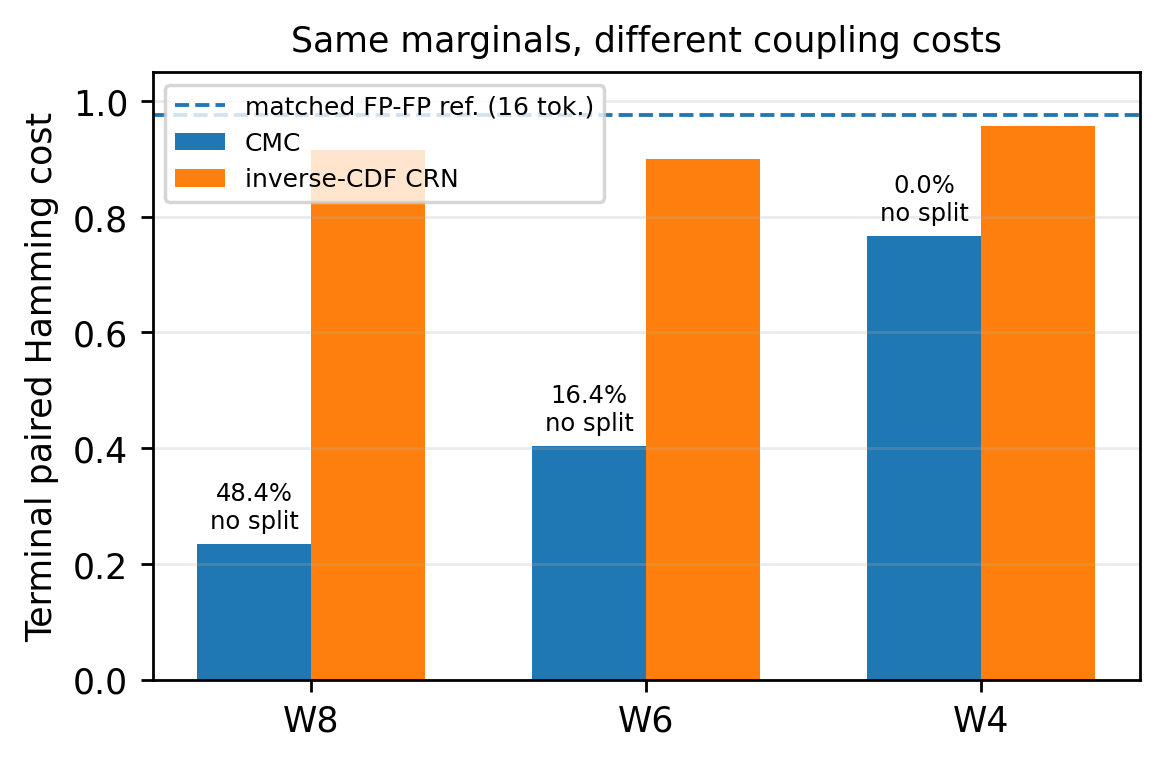
\includegraphics[width=\linewidth]{figures/figure_main_coupling.png}
\end{minipage}\hfill
\begin{minipage}[t]{0.49\linewidth}
\centering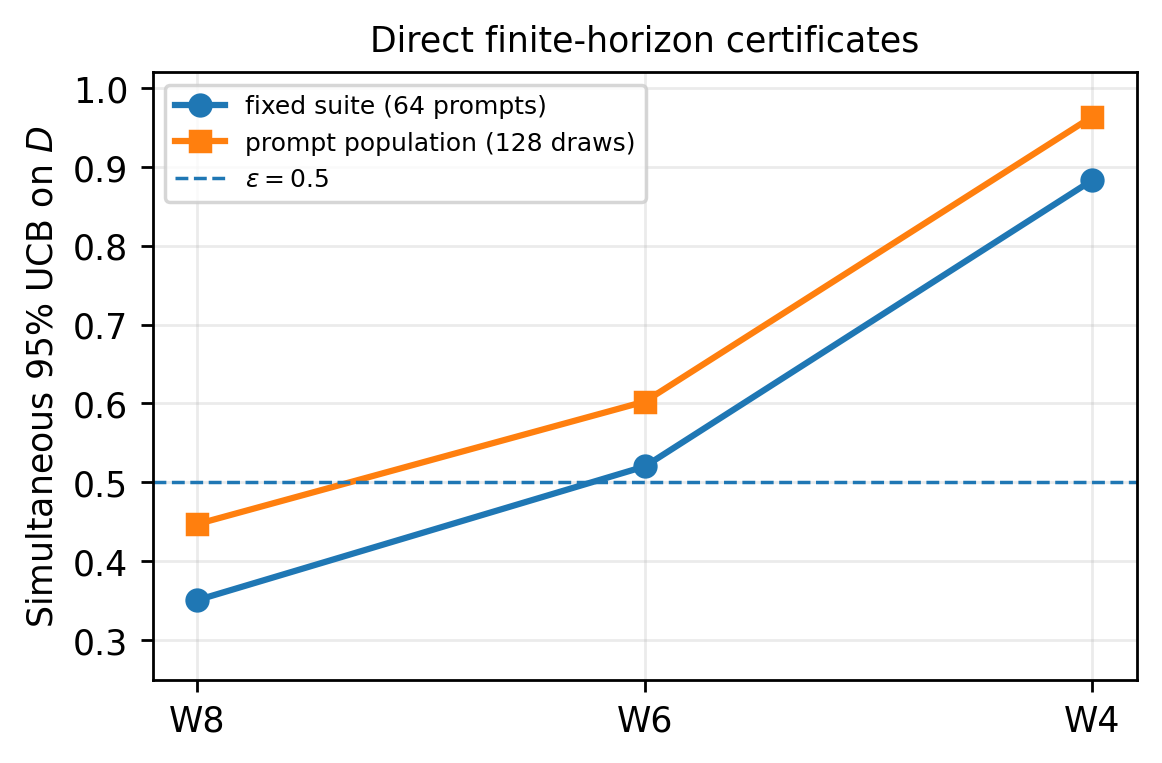
\includegraphics[width=\linewidth]{figures/figure_main_certificates.png}
\end{minipage}
\caption{\textbf{Left:} changing only the coupling changes the measured terminal cost. \textbf{Right:} direct simultaneous UCBs on the fixed suite and declared prompt population. A UCB above $0.5$ means that tolerance $0.5$ is not certified at full horizon; it is not a validity failure.}
\label{fig:main-results}
\end{figure}

The population panel preserves the aggregate precision ordering, but its estimand differs. At W8, trajectory-draw split probability changes from $0.5156$ on the fixed suite to $0.5781$ under the source-population experiment; trajectory-conditional endpoint damage changes from $0.455$ to $0.490$. Prompt-block any-split fractions ($0.805/0.969/1.000$) are reported separately and are not trajectory split probabilities.

\paragraph{Sensitivity to the within-prompt independence premise.}
The fixed-suite primary radius treats the four event-addressed coupling streams per prompt as independent bounded draws, as preregistered. A conservative prompt-block analysis first averages those draws and uses only $m=64$ blocks, doubling the radius from $0.11598$ to $0.23197$. The corresponding W8/W6/W4 direct UCBs are $0.4668/0.6363/0.9991$: W8 remains below $0.5$, whereas W6 and W4 weaken. We report both analyses because the primary statement relies on the standard idealization that independently addressed pseudorandom streams implement independent Monte Carlo draws.

\subsection{Incidence and consequence of the first split}
\label{sec:mechanism}
The first-divergence decomposition predicts two distinct quantities: how often a split occurs and how much unresolved suffix remains when it occurs. The data support that separation. Lower precision increases common-state mismatch incidence, while the same split is much more consequential early in reverse time than late (Figure~\ref{fig:mechanism}).

\begin{figure}[t]
\centering
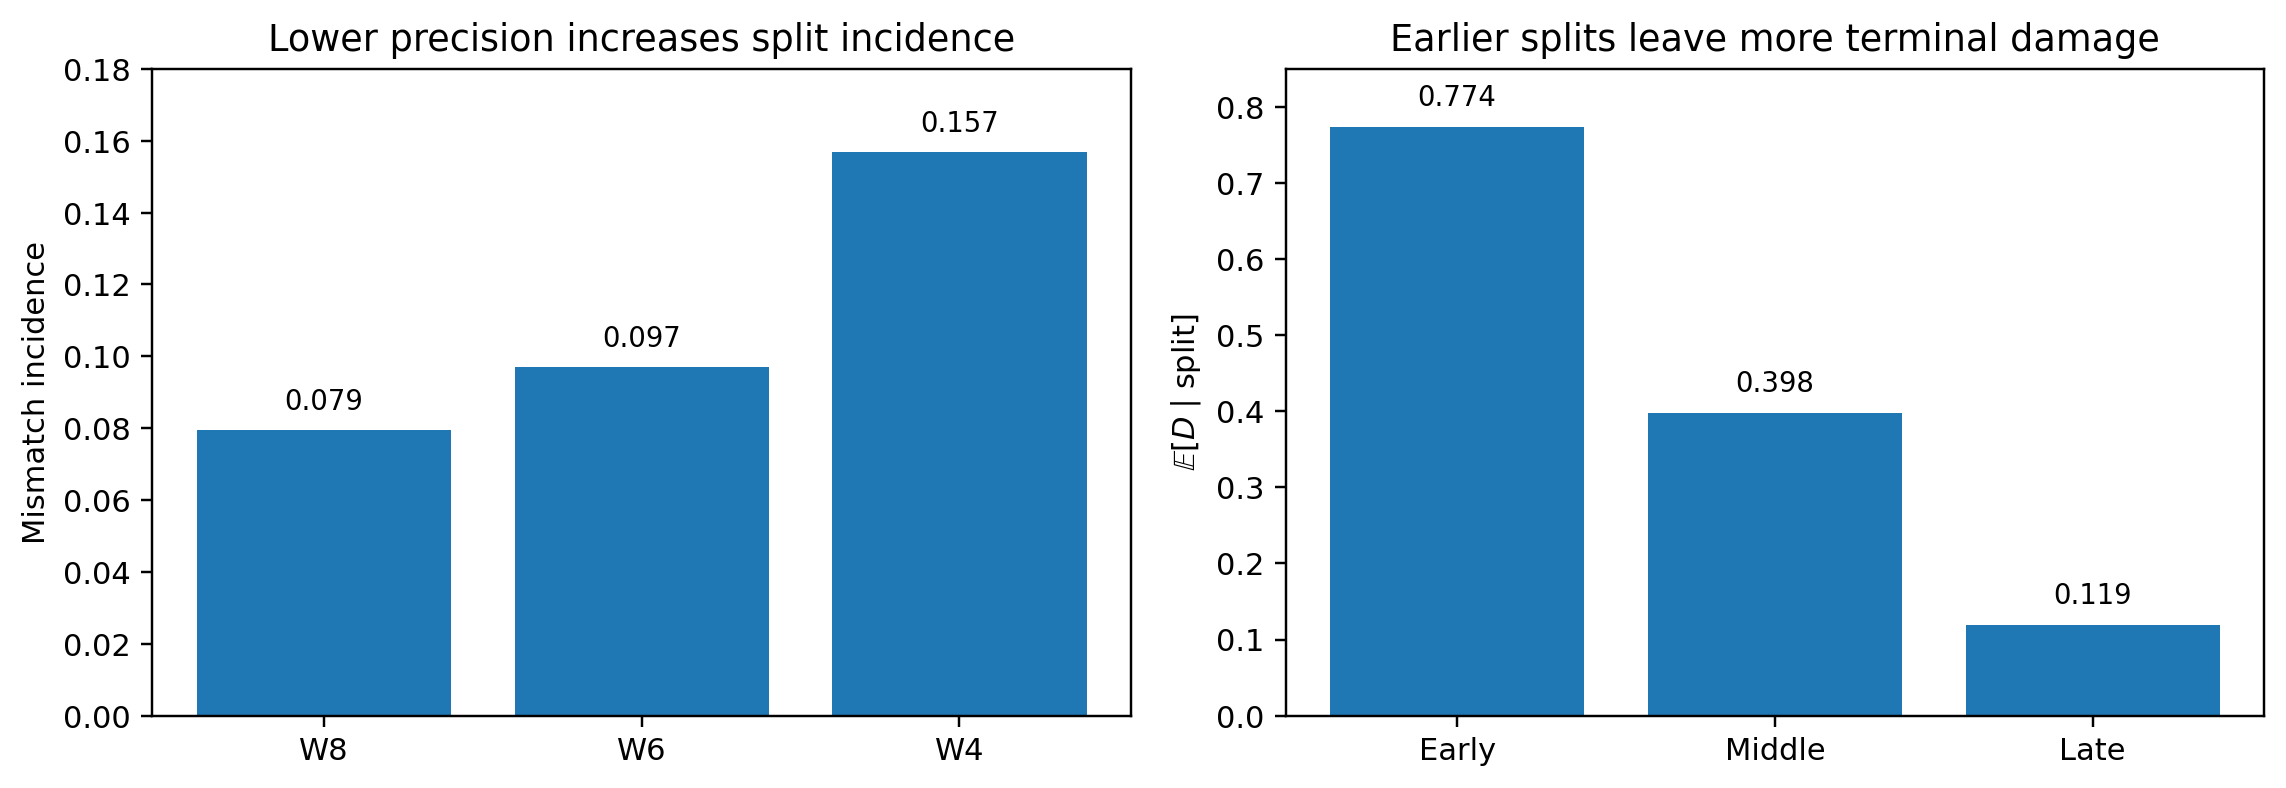
\includegraphics[width=.92\linewidth]{figures/figure_mechanism.png}
\caption{Mechanism behind terminal damage. \textbf{Left:} lower precision raises same-state mismatch incidence. \textbf{Right:} conditional terminal damage after an early split is far larger than after a late split.}
\label{fig:mechanism}
\end{figure}

The W8/W6/W4 mismatch incidences are $0.079/0.097/0.157$. Conditional terminal damage is $0.774$ for early, $0.398$ for middle, and $0.119$ for late splits. These values give empirical content to Equation~\eqref{eq:hazard}: bit width primarily changes the split hazard, while remaining masked mass and suffix length control the consequence. The identity is descriptive rather than an optimization theorem; Appendix~\ref{app:negative} reports a preregistered calibration attempt that failed to turn this decomposition into a task-improving method.

\subsection{Finite-bit scaling, model transfer, and task relevance}
A preregistered 32/32 calibration/held-out study evaluates W3--W8 on fresh prompt draws. Over the prespecified W4--W8 fit range, held-out prompt-fixed-effect slopes are
\[
\beta_W=0.7855\ [0.7618,0.8078],\qquad
\beta_H=0.7580\ [0.7346,0.7804],
\]
for exact one-step Wasserstein cost and CMC split hazard; within-prompt $R^2$ exceeds $0.96$. W3 is a preregistered stress point and is excluded from the primary fit. These are finite-range empirical summaries, not asymptotic quantization laws.

On a separate 1.14B SMDM checkpoint, direct CMC costs increase with lower precision at both 16 and 64 generated positions. Full-horizon direct UCBs at length 16 are $0.433/0.677/0.947$, and at length 64 are $0.599/0.807/0.993$ for W8/W6/W4. A separate 100-example GSM8K panel gives BF16/W8/W6/W4 accuracies $51/51/50/49\%$ with exact McNemar $p$-values $1.000/1.000/0.625$. It is deliberately described as task relevance evidence rather than a coupling certificate because that archived task run did not record a valid proposal coupling. The contrast between large exact-token CRN cost and unchanged W8 accuracy is one reason we do not interpret Hamming as a semantic or task-performance metric.

\subsection{Official sample-then-select sampler}
The SMDM task sampler first samples position-wise candidate tokens and then applies a global fixed-count confidence top-$k$ decision. We couple proposals and push them through the unchanged FP and quantized selectors. At temperature zero the proposal law is deterministic and coupling choice disappears, as predicted by Corollary~\ref{cor:det-limit}. At temperature $0.2$ the pushed-forward law is nearly deterministic. Raising temperature creates measurable support after selection: at temperature $1.0$, maximum empirical effective support is $1.449$ and minimum modal probability is $0.817$.

\begin{figure}[t]
\centering
\begin{minipage}[t]{0.64\linewidth}
\centering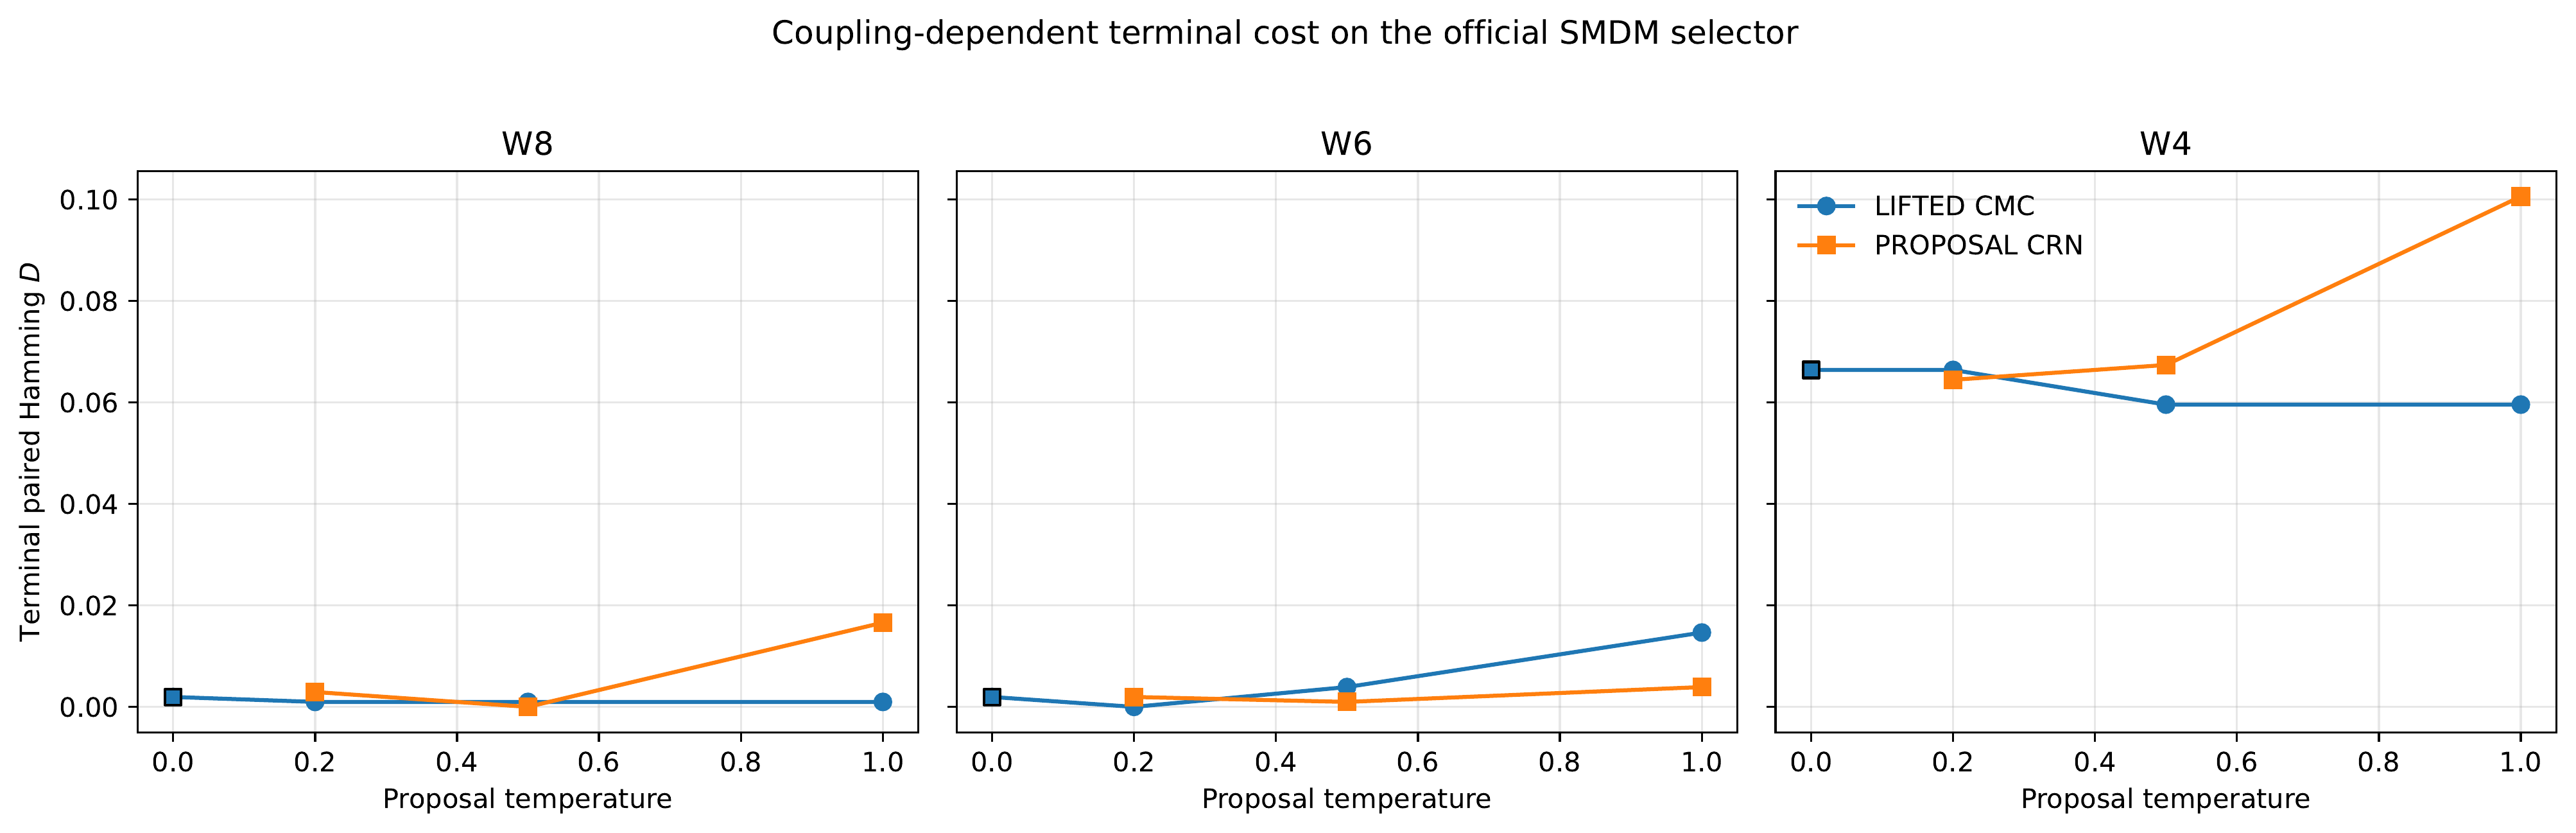
\includegraphics[width=\linewidth]{figures/figure_temperature_coupling_cost.png}
\end{minipage}\hfill
\begin{minipage}[t]{0.34\linewidth}
\centering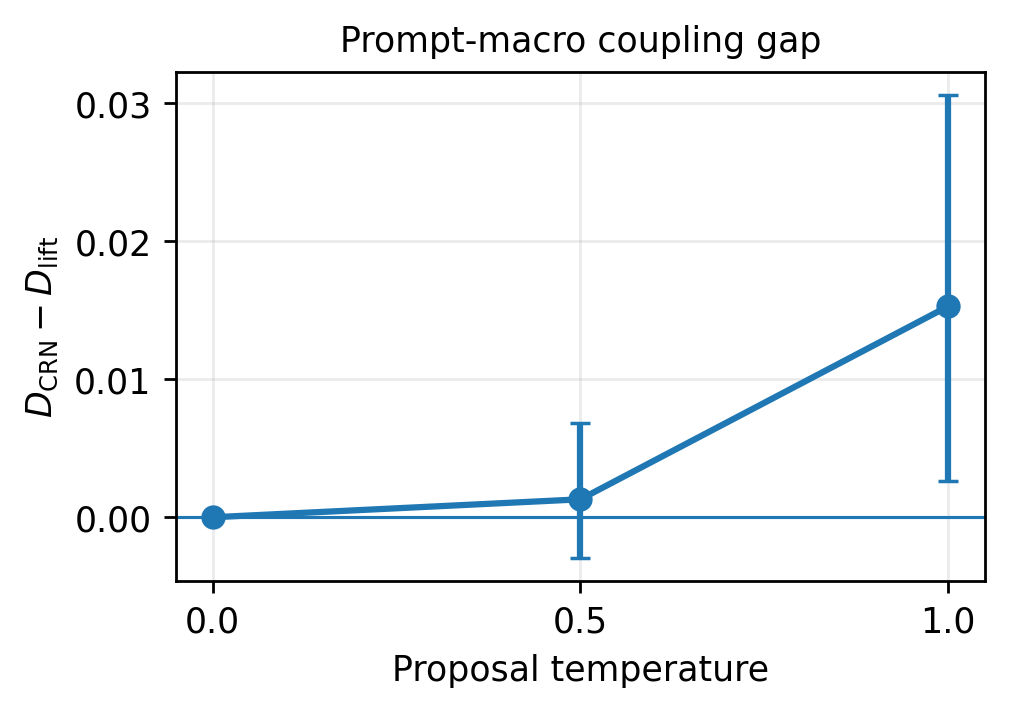
\includegraphics[width=\linewidth]{figures/figure_temperature_gap_compact.png}
\end{minipage}
\caption{Coupling dependence on the official sampler. \textbf{Left:} terminal cost by bit and proposal temperature. \textbf{Right:} prompt-macro $D_{\rm CRN}-D_{\rm lift}$ with paired prompt-cluster bootstrap intervals. The mean gap is positive at temperature $1.0$, but bit-level directions are mixed.}
\label{fig:temperature}
\end{figure}

At temperature $1.0$, the prompt-macro CRN-minus-lifted gap is $0.0153$ with bootstrap interval $[0.0026,0.0306]$, but the median gap is zero, the one-sided sign-test $p$-value is $0.166$ (Holm-adjusted $0.332$), and W6 reverses direction. Lifted CMC reduces proposal-vector mismatch from $0.1709$ to $0.0724$, yet post-selection next-state mismatch remains nearly unchanged ($0.0142$ versus $0.0146$): the selector maps many different proposals to the same next state. Conditional healing is also mixed across bits. Thus coupling dependence survives outside the deterministic limit, while proposal-level maximality does not induce a universal terminal-cost ordering.

\subsection{What the certificates do not establish}
All preregistered relative-to-reference-diversity certificates fail. First-divergence bounds can be loose because they intentionally ignore post-split healing. Exact-token Hamming is auditable and aligned with the theory, but it is not a semantic-quality certificate. The next section reports two preregistered investigations designed to test stronger interpretations; both return negative results.
